\chapter[Text classification]{Text classification}
\label{ch:text-classification}
   

%In the 1960s, if you wanted to read the news, you bought or borrowed a newspaper. If you were unwilling to spend the necessary time, you could read capsule summaries of the most important news in, for example, \mediatitle{Time} magazine's Listings section. If you were too busy, or too important, to do even that, you could arrange for someone to read the newspapers for you and give you a summary of what you needed to know.  If you were a fruit-grower, you could subscribe to \mediatitle{Fruit Growers' News} and get targeted digests of the news that mattered to you.

%But now, many newspapers and magazines offer you the chance to read their material online, often at no charge. This is a big change, because the text is now searchable, indexable and available for reuse. As well as traditional newspapers, there are weblogs and \keyword{aggregator sites}.  Aggregators pull together information from all over the web, providing a digest suitable for the target audience.  Aggregators exist for tracking news about cars (\url{http://www.autoblog.com}), greener cars (\url{http://green.autoblog.com}), bicycles (\url{http://www.cyclelicio.us}), running (\url{http://www.coolrunning.com}), baby strollers (\url{http://strollersandprams.com}) and stationary exercise machines (\url{http://www.treadmilladviser.com}). Even \mediatitle{Fruit Growers' News} is now readily available  online (\url{http://www.fruitgrowersnews.com}), as are countless other websites and weblogs catering to specialist interests. These can be money-making  ventures if they can deliver an audience that is attractive to advertisers.


% NEW OUTLINE.
% what is document classification?


% training data, data cleaning (?), labels, feature extraction, machine learning, evaluation.
% let's walk through it with Naive Bayes and Spam.
% Perceptron.
% which algorithm to use?
% What are you going to do with this information? Payoffs. Epidemiology.
% do you want to deploy something commercially or just better understand your data?
% harder cases and why are they hard? 
% negation
% sarcasm
% assholes on reddit/amI the asshole, 
%author gender,
% resumes classified as what we want or not....college application essays....
% fake news or real news, personal attack (moderated comment) or not, 

\section{Introduction}

Every day, you probably receive hundreds of \keyword{spam} emails -- unsolicited advertisements, financial scams, and attempts to steal personal data -- which your email automatically sends to your spam folder so you don't even see them. Your email \keyword{spam filter} is one example of \keyword{text classification} (also called \keyword{document classification}): When a computer automatically sorts texts into two or more \keyword{classes}, also called \keyword{labels}.  Here, the texts/documents are emails, and the classes/labels are ``spam'' (junk, named after a sketch by the British comedy troupe Monty Python) and ``ham'' (the real emails that you want to read).  

Spam detection is just one example of text classification.  Other popular applications include:

\begin{itemize}
    \item Sorting your non-spam email into folders -- primary, social, promotions, and forums  (note that we can use as many classes as we want).
    \item Detecting hate speech or fake news in online posts, perhaps to  delete it automatically (\keyword{content moderation}; here, the texts are the posts,   the classes are ``hate speech'' and ``not hate speech,'' or ``fake news'' versus ``real news'' -- note that these categories may be somewhat subjective).
    \item Classifying a product review as  positive, negative, or perhaps also neutral (\keyword{sentiment analysis}).
    \item Detecting the language that an online post is written in (\keyword{language identification}) -- English, Spanish, Tagalog, and so on.  Here, the number of classes is determined by the number of languages that we want to handle.
    \item Classifying the type of issue that a customer needs help with (\keyword{support ticket classification}) -- orders, shipping, returns, other -- to send them to the right agent or help page.
    \item Identifying what a language technology user wants to do based on what they say or type (\keyword{intent recognition}) -- do they want to shop, set a timer, do a calculation, translate something into another language, look at maps, or view general search results? 
\end{itemize}

Text classification is used any time you want to assign a label  automatically to a text from a closed class of labels.  Beyond business applications, it can be used in language research of all kinds, including linguistics, computational social science, and digital humanities.  We illustrate with spam because it is simple, familiar, and arguably binary (with just two labels, spam and ham). But even if you don't care how your spam filter works, learning about text classification will empower you in all areas of language processing.


\section{Exploring the data} 

Before learning about how computers classify spam, it may be useful to look at some examples of spam and ham, taken from the inbox and spam folder of one of our own email accounts.  It is always a good idea to understand the data yourself before you feed it to an algorithm.

\begin{itemize}
    \item  Better than Morphine, Safer than Aspirin?
        \begin{itemize}
                  \item  Little did they know, a Columbia University MD already found the ``Holy Grail'' back in the 1970s. You see, this doctor uncovered a powerful, natural painkiller... that works with your body's natural mechanisms to renew your achy joints from the inside out.
        \end{itemize}
    \item  Click Here for your \$1000 Gift Card
        \begin{itemize}
                \item  I am Mr Roth Savuth and a personal Accountant Director with Foreign Trade Bank of Cambodia (FTB). It is with good spirit of heart that I open up this great opportunity to you.
        \end{itemize}
    \item  Attention Sir/Madam
        \begin{itemize}
                \item  From the outset, I wanted the very fabric of my club to be built around support. For the most part, I deal exclusively with our most valued clients.
        \end{itemize}
    \item  Reminder: Course Instructor Opinion Survey (CIOS)
        \begin{itemize}
                \item  The course/instructor opinion survey (CIOS) is now underway for one or more of your courses. The CIOS tool is an important source of information about your teaching and can be very helpful for classroom professors.
        \end{itemize}
    \item Request for a reference letter
        \begin{itemize}
                \item  I hope you're doing well, and apologies for not having replied to your last email on sociolinguistics next semester! The last half of the semester became a lot busier than I anticipated. 
        \end{itemize}
    \item  Question about final project
        \begin{itemize}
                \item  I saw in the announcement that we might submit the final write-up before December 8th, but I still want to clarify if the deadline is on the 7th or before the end of the 8th.
        \end{itemize}
    
\end{itemize}



You can probably tell at a glance which of these emails are spam or ham (the first three are spam, the last three are ham). But how did you do that? What clues did you notice?  And how did this email client already correctly sort them into spam and ham?

%One of the most commercially significant uses of this technology is known as \keyword{sentiment analysis}. Another term that means much the same thing is \keyword{opinion mining}. The key idea is to automate the detection of positive and negative sentiments in documents. For many years companies, political parties and pressure groups have used focus groups and audience surveys to track  opinions about their products, policies and positions. Sentiment analysis technology promises to be able to automate this process, trawling the press, internet and social media for documents that express opinions,  organizing them according to the opinions that they express, and presenting summaries of the results.  This is a kind of \keyword{data mining}, one that makes especially heavy use of language technology.

%For example, if you want to find out about the general opinion of the movie  \mediatitle{Pearl Harbor}, you can check out Metacritic (\url{http://www.metacritic.com}) or Rotten Tomatoes (\url{http://www.rottentomatoes.com}) and see multiple reviews, by both professionals and lay people. The least favorable user review makes its opinion very clear: \begin{quotation}\noindent Ridiculous movie. Worst movie I've seen in my entire life [Koen D. on metacritic] \end{quotation}

%The person hates it. The most positive review is equally clear:
%\begin{quotation}\noindent
%One of my favorite movies. It's a bit on the lengthy side, sure. But its made up of a really great cast which, for me, just brings it all together. [Erica H., again on metacritic]
%\end{quotation}
%but for this movie, most of the reviews are similar to  Alan Scott's from the New York Times : \begin{quotation}\noindent The Japanese sneak attack on Pearl Harbor that brought the United States into World War II has inspired a splendid movie, full of vivid performances and unforgettable scenes, a movie that uses the coming of war as a backdrop for individual stories of love, ambition, heroism and betrayal. The name of that movie is \mediatitle{From Here to Eternity}. (First lines of Alan Scott's review of \mediatitle{Pearl Harbor}, New York Times, May 25, 2001) \end{quotation}

%While Scott's review finishes up being positive about the fabulous action sequence at the heart of \mediatitle{Pearl Harbor}, and very positive  about \mediatitle{From Here to Eternity} (a different, and apparently much better, movie),  it drips with sarcasm about everything else in the movie.  That is obvious to a human, but is difficult for a machine to spot.

% Here is another review that we enjoyed reading: \begin{quotation}\noindent
%The film is not as painful as a blow to the head, but it will cost you up to \$10, and it takes three hours. The first hour and forty-five minutes establishes one of the most banal love triangles ever put to film. Childhood friends Rafe McCawley and Danny Walker (Ben Affleck and Josh Hartnett) both find themselves in love with the same woman, Evelyn Johnson (Kate Beckinsale). [Heather Feher, from \url{http://www.filmstew.com}]
%\end{quotation}

%Most review sites use human editors to associate scores with reviews, but this is very much the kind of thing that people want to automate. Some of the automation might be quite easy: a review that dubs the film \exsent{Ridiculous} and \exsent{Worst} is probably negative, and  one that says \exsent{Favorite} and \exsent{great} is probably positive. But Scott's clever \mediatitle{New York Times} review reads a lot like a very positive review, until you notice that the positive comments are directed at a completely different film. And Feher's backhanded \exsent{not as painful as a blow to the head} is also likely to defeat any simple automated system.

%\exsent{Painful} would be bad, \exsent{not painful} might be good, \exsent{not as painful as \ldots } suggests that some pain is involved. \exsent{Not as  painful as a blow on the head} quantifies the pain in a rather alarming way.  Language is like that: the meaning twists and turns as each word is  added to the next. The authors happen to find Feher's subtle deployment of this roller-coaster  effect cool and funny, but it certainly is not going to be easy for a machine to handle.

%Clearly, if we can rate movie reviews automatically, we can make our own versions of MetaCritic, and maybe apply the idea to a wider range of things than is possible when humans are in the loop.  But language is subtle, so we can't be sure that this kind of automation is going to be possible. 

%The movie sites are interested in telling the difference between good and bad reviews, and also in assigning a numerical score -- which generally makes them semi-structured data, as outlined in chapter~\ref{sec:semi-structured}.  In general, when we are interested in assigning a label (e.g., \emph{good} or \emph{bad}) to a document, the task is called \keyword{classification}. In this chapter, we focus on document classification, and show some of the uses to which it can be put. The most important practical examples of this technology are the junk mail filters that try to protect you from the flood of unwelcome email that would otherwise clog up your inbox. These things are so good that we normally hardly notice them, but when they stop working or misbehave we realize how important they are in keeping our email interactions manageable. Other uses of the technology are call routing systems (the systems that try to send you to the best, or perhaps cheapest, person when you phone a helpline), systems for classifying texts by topic, and systems that classify documents according to their \keywordAs{sentiment}{sentiment classification}. An automated movie review site would need a really good sentiment classifier to judge whether a review is good or bad. It might also make use of a topic classifier to scan documents and decide whether they are movie reviews in the first place.

\section{How computers ``learn''}

Text classification represents one  example of \keyword{machine learning} -- any task in which the  computer is expected
to ``learn'' from experience. 
If we wanted, we spend pages discussing whether machines can ever be said to be truly intelligent, 
or  about the true nature of the so-called learning. 
We think these discussions are interesting, and we touch on them very briefly at the end of Chapter~\ref{ch:dialog-systems},
but they really belong in a philosophy class, not here. 

There are several different types of tasks that machine learning models can ``learn'' to solve.  Text classification is an example of a \keyword{classification} task: The model is asked to assign the text a class/label, from a closed set thereof.  Classification is known as a \keyword{supervised learning} task because the model is trained on data that has already been labeled with ``correct answers'' and just needs to learn to  label new data in the same manner. 
% also regression (supervised), clustering, 

In a classification task, we have access to a labeled \keyword{training set}  -- a set of emails correctly labeled as  spam or ham.  Where did the labels come from?  Perhaps the labels were gathered opportunistically from users who helpfully flagged some emails as spam or immediately deleted them (spam), while reading and replying to other emails (ham).  Perhaps the researcher paid  gig workers to label the emails through a platform such as Amazon's Mechanical Turk.  

Next, we have to turn these emails into some sort of representation that the computer can process.  As we discussed in \chapref{ch:textasdata}, numbers are more meaningful to a computer than text, because numbers can be manipulated (added, multiplied), and the distance between them can be quantified.  So we need to turn our documents into vectors of numbers, in such a way that the numbers represent something meaningful about each document -- the information that you need to classify it as spam or ham.  This process is also known as \keyword{featurizing} the document -- creating a computer-friendly vector representation of the \keyword{features} of the document that are important for the classification task.

There are all sorts of ways to featurize a document, some very fancy and complex, but one very simple way is just to count the words. To illustrate, imagine that we have three very short emails to featurize:

\ea \ea Email1: Better project idea
    \ex Email2: Better than morphine
    \ex Email3: Project question
\z 
\z 

In this simple example, we have a vocabulary of six word types (\exword{better, project, idea, than, morphine, question}). We can represent each document as a seven-element vector, where each position in the vector corresponds to a word in the vocabulary, and each value reflects the number of times that this word occurs in the document.  Putting the emails together into a matrix, we end up with a \keyword{term-by-document matrix}: Each document (email) is a column,  each term (word type) is a row, and each value reflects the frequency of that term in that document.


\begin{table}
\begin{tabular}{lccc}
\lsptoprule
       & Email1 & Email2  & Email3 \\ \midrule
better & 1 & 1 & 0 \\
project & 1 & 0 & 1 \\
idea & 1 & 0 & 0 \\
than & 0 & 1 & 0 \\
morphine & 0 & 1 & 0 \\
question & 0 & 0 & 1 \\
\lspbottomrule
\end{tabular}
\caption{Term-by-document matrix for three short emails.}
\label{fig:term-by-email}
\end{table}


 Reading these three emails, you probably get the sense that Email1 and Email3 are more similar to each other than they are to Email2.  For one thing, Email2 seems like spam because it is about drugs, whereas Email1 and Email3 seem legitimate because they are about projects.

Notice that our simple term-by-document matrix already captures this intuition!  Just by comparing which columns match on a given row, we see that Email3 is more similar to Email1 (since both of them contain the word \exword{project}) than to Email2 (which has no words in common with Email3).  There are mathematical ways to compute the similarity between two document vectors, which we explore later in the book, but the important point is the big picture, previewed in \chapref{ch:textasdata}: When we represent a document as a vector, we capture something about its contents and its similarity to other documents.

This term-by-document matrix representation is called a \keyword{bag of words} because it does not represent any information about the order of words, just their frequency.  Imagine writing a sentence on paper, then chopping up the paper into individual words and tossing them into a bag, so that no word order is preserved. Setting aside everything we learned about grammar in \chapref{ch:writers-aids}, we ignore the fact that the words were arranged into a particular order and that they go together to form sentences and paragraphs.  All we worry about is which words happen in the document and how often they happen.

Even though this representation is simple, we face all sorts of design choices: Should the words all be put in lower-case?  Should we include emoji?  Should words be lemmatized (mapping \exword{dog} and \exword{dogs} to the same form)? Should we remove stop-words such as \exword{the}, or down-weight their importance? Should we focus on the presence/absence of specific, important words or look at all of them?  Should the researcher use their own judgment to decide what features are important (\keyword{feature engineering}), or leave the computer to figure it out?  There are pros and cons to each choice.

Once we have our vectors of features, we want the computer to learn how to map these feature vectors into the correct labels for spam and ham.  There are many different algorithms for teaching the computer to do this; we will explore two simple ones in detail below (naive Bayes and the Perceptron).  Through this process, the computer produces an object called a \keyword{model}, a representation of what it has learned.

Our next step is to test how successful our model is.  Our measure of success should be tied to the ultimate goal of the model -- to classify new emails, for which we do not yet know the correct label.  But if we do not know the correct label, then we do not know whether our model is labeling them correctly.  Instead, we use a \keyword{test set} of  examples, for which we ourselves know the correct label, but the model does not.  It is common to split off part of the original labeled data (10-20 percent of it), exclude it from the training data, and save it for later as a test set.  We can then feed the test set to the model and compare the model's predicted labels to the correct labels.

% why not just look at the training data?

Here, you might wonder: Why not just test the model on the same data that it was trained on?  But the goal is to build a model that can generalize to new data, eventually including those for which we do not even know the correct label.  So we want to test whether the model's success can generalize beyond the data that it has already seen.  Otherwise, we run the risk of \keyword{over-fitting} -- building a model that has memorized  the correct labels for the training data, so that it performs very accurately on those examples but falls apart when it sees something new.  

To use an analogy, imagine that you are preparing for a test in your linguistics class.  Your friend shows you the test that was given in the class last year, along with the correct answers to that test.  You could decide to just memorize last year's test and its answers.  If the instructor is too lazy to write a new test this year, you will do well -- but you will not have actually learned much linguistics; your knowledge will be \exword{over-fitted} to this particular test.  On the other hand, you could use last year's test as a study guide, and learn the key concepts taught in the class; this way, you will do well on this year's test even if it differs from last year's -- and, most importantly, you will have actually learned some linguistics concepts which you can generalize to various problems.  By testing the model on new data, we check whether it has learned to generalize.

The final step is to deploy the model in real life, where its job is to label new data for which we do not know the correct label.  The model can be incorporated into an email service as its spam filter.   If the model works well on our test data, can we expect it to work equally well in real life?  That depends on whether the real-life data are similar to the data on which the model was trained and tested.  If spammers start to realize what features are sending their messages to the spam folder, they may start to create spam that is harder to detect.


% how similar are the real world data to the training and test data?




% circle back to: other types of machine learning; 
% ethics
% how similar is the real life data to the training/test data.

% featurizing 

%Our ultimate goal is to learn from the training data in order to build a robust system that can process future examples of the same kind as those that we found in the training set -- new, unseen emails. Clearly, we have a problem, because future examples are not yet available.

%As an approximation, we use a separate \keyword{test set} of examples to stand in for the unavailable future examples. Think of these as this month's \mediatitle{New York Times} articles. Since the test set is separate from the training set, the system will not have seen them. If the system performs well on the test set examples, it will probably also do well on the unseen future examples.

%There are several important variations on this scheme, which we take a closer look at in the next sections.

%\subsection{Supervised learning}
	
%In \keyword{supervised learning} we need the training set and the test set to have been labeled with desired ``correct answers''. Imagine that there is a news service that provides a stream of uncategorized articles, and that a newspaper needs a system that will sort these articles into separate piles for \emph{News}, \emph{Sport}, \emph{Arts}, \emph{Business} and \emph{Do not use}. The first step is to make a training set and a test set by labeling a few hundred articles with the desired categories. The second step is to apply machine learning software to the labeled training set. This produces an object called a \keyword{model}, which summarizes what the software has learned from the training set. 

%The third step is to read the learned model into the machine learning software and use it to generate \emph{predictions} for the test set. Since we are testing the model's ability to make a prediction, we do not let the software see the correct answers for the test set examples. If the software is working well and the model is good, the predictions will often be accurate. We discuss precisely how to measure accuracy in section~\ref{eval:sec}.  It is unlikely that the model will be perfect, but it may well be good enough. 


%The fourth and final step is to deploy the learned model on unseen examples. It uses what it has learned to sort the articles into the necessary piles.
%	This kind of learning could be the basis for an automated system. A newspaper might have a national news section, a local news section, a business section, and a sports section. The learning goal would be to  allocate each article to the correct section.
%In a real-world application, there will usually be someone who is responsible for checking the results before the paper is printed, because there will almost certainly be some mistakes, no matter how good the machine learning method is.
	
%\subsection{Unsupervised learning}

%In \keyword{unsupervised learning}, we assume that there are no pre-specified categories. Imagine that the newspaper still gets a stream of uncategorised articles, but now the task is to organize the articles into piles in such a way that {\bf similar} articles occur in the same pile. In this setting, the piles are often called \keyword{clusters}, and the process of organizing the articles into clusters is called \keyword{clustering}.  Clustering can be used to sort articles into groups that could be laid out on the different webpages of an online publication.  In that setting, there is no need for the groups to have fixed names.

% The reader will be able to notice that articles in a given cluster share something, such as being about sports, but the algorithm would be just grouping articles, not trying to name the clusters. The big plus of this approach is that you do not need a training set, so there is no costly process of going through labeling up the articles. The big negative is that the clusters might not be that intuitive. For example, if you cluster common words, one cluster often turns out to be the words \exsent{Monday}, \exsent{Tuesday}, \exsent{Wednesday}, \exsent{Thursday}, with \exsent{Friday} off in another cluster. This is because Friday is the only weekday that frequently turns up following \exsent{Thank goodness it's \ldots}.

%\section{Features and evidence}

%When we try to classify or cluster documents, the first step is to identify the properties that are most relevant to the decision that we want to make.  These properties are called \keywordAs{features}{feature}. In biology, a specimen could have features like scales or gills. If you observe these features, you can be fairly confident that your specimen is a fish. In the same way, when you are trying to decide whether a document is  junk mail or not, you should pay attention to features of the document that are likely to help with the decision.

%If you are trying to guess whether something is junk mail, these could  include things like:
%\begin{itemize}
%\item Whether the document mentions a large sum of money. 
%\item Whether the greeting used in the document is something weird
%  like \exsent{Respected Madam} or not.
%\item Whether there are non-standard honorifics like \exsent{DR. MRS.} or not.
%\item Whether it has words written entirely in upper-case or not. (If the whole message is in upper case, then you might want to think that the writer was angry, or a little crazy, but that is a feature which is not very relevant to junk mail detection).
%\item Whether the document uses the words \exsent{Viagra}  and \exsent{sex} close to each other.  \end{itemize}

% None of these features are certain indicators of junk mail, but all are strong evidence that the document is more likely to be junk than if we had
% not seen the feature. To make a useful system, we need to tell the computer two things. First, we have to say exactly which features are used and exactly how to detect them. Second, we have to specify a way of weighting the evidence provided by the features. It often  works well  to use machine learning to weigh the evidence, rather than doing it by hand, but it is much harder to automate the first stage of deciding what evidence is potentially relevant.  This first stage is often called \keyword{feature engineering}.

%There are two common strategies for doing feature engineering.  The first is to use lots of features, in the hope that some of them will be relevant and useful.  We will call this the \keyword{kitchen sink   strategy}, since we throw everything we have at the problem, including, perhaps, the kitchen sink.  If you are building a junk mail detector, you could adopt a version of this strategy by using the words themselves as features: because there are lots of different words in the messages, there will also be lots of different word-based features. It is almost certain that some of these features (such as the presence or absence of the word \exword{enlargement}) will be useful indicators. Of course, there will also be many irrelevant features, such as the presence or absence of the word \exsent{apple}. If we adopt the kitchen sink strategy, we will need to choose a machine learning method that is good at focusing on the few but important relevant features, and also good at ignoring the many irrelevant features. We will return to this later in the chapter, when we discuss machine learning methods in detail.

%Feature engineering actually has two parts. You need to decide which features you would like to collect, then write computer code to actually do the work of collecting them. One advantage of using words as features is that it is almost as easy to collect and count all the words in a document as it is to collect just a selected few. 

% The second common strategy for feature engineering is to use careful thought to try to identify, ahead of time, a small set of features  that are likely to be relevant. We will call this the \keyword{hand-crafted} strategy, because it demands from the software developer the same kind of careful and sustained attention to the problem that a skilled woodworker might  give to the creation of a beautiful piece of furniture. The software developer uses intuition and experience to select features that seem promising An advantage of this approach is that there will be fewer irrelevant features, so the machine learning method does not have to be as good at ignoring them as was needed when we were using the kitchen-sink features. A disadvantage is that the  task of choosing relevant features ahead of time is very difficult.  Human beings are not good at this task.  Part of the reason is that it is hard to know whether the selected features are general enough. Testing for \exsent{DR. MRS.} specifically is easy, but it is far harder to cover all the cases of similar things that might arise.

%In practice, most software developers use an \keyword{iterativ   method}. They pick an initial set of features, train a classifier, measure how well it does, then try to work out which features are working well, and which less well. By analyzing the results, they come up with ideas for further features, add them in, and retry the machine learning. Depending on the problem, they might go around this cycle multiple times, until satisfactory performance is reached. The key to the success of this iterative  approach, which is used on a much larger scale by firms such as Google, is to insist on systematically and thoroughly measuring success rates. With the luxury of very large numbers of users and correspondingly huge data centers, the big web firms can rapidly collect evidence about how well they are doing. This instant feedback makes it possible to try out all kinds of possible improvements, keeping only the ones that seem to work well. 

%Software developer time is a limited resource,  so it may be better to quickly collect a large number of easy  but marginally relevant features than to spend a lot of time  trying to write code to extract   the difficult features. 

%\section{Application: Spam filtering}

%The Text Retrieval Conference (TREC) made available a sample collection of email consisting of about 57,000 junk emails and about 39,000 good emails. Computer scientists and engineers tend to call junk emails \emph{spam}, for reasons that are slightly unclear, but which may involve the obsession that the Monty Python comedy team had with Hormel's processed pork product. They also tend to call non-junk emails \emph{ham}, presumably on the basis that real ham is to be preferred to any imitation.  The authors feel that the spam/ham terminology is a bit geeky, and try to avoid over-using it, but sometimes we cannot help ourselves.

%When writing this paragraph,  we checked and found that one of us had received 20 spams and 3 hams in the last 12 hours.  All the spam was successfully filtered out.  Many people (including us) trust the filters enough to hardly ever check for misclassified ham.  We say that the \keyword{false positive rate} of the spam detection task is very low (see more below on measurements).

\section{Measuring success}
\label{eval:sec}

How do we decide whether our spam-detection model is successful?
It may seem obvious what we need to measure. If we classify all the spam as spam and all the ham
 as ham, we have succeeded and all is well. This is definitely
correct, but we would be fooling ourselves if we believe that we
can design a perfect system that gets 
every single decision correct. 
Therefore, we need measures that quantify our partial 
successes and failures, so we can weigh their trade-offs.



To do this, we borrow some ideas from medical science. These ideas apply
anywhere, but they turned up first in medicine because of the need to
reason effectively with complex and uncertain data.  When we run a
classifier on a document to decide whether it is spam or not, it is a
lot like running a diagnostic test to collect evidence about whether a
patient has a disease or not. Here there are two two-way distinctions
to be made:

\begin{enumerate}
\item
The test can come out either positive
or negative.
\item The patient may or may not really have the disease.
\end{enumerate} 

So there are four possible ways that the situation could be after the
test has been given, as shown in \tabref{tab:diagnostic}. 


\begin{table}
\begin{tabular}{lcc} 
\lsptoprule
& \emph{Has disease} & \emph{No disease} \\ \midrule
\emph{Test positive} & True positives & False positives \\
\emph{Test negative} & False negatives & True negatives \\
\lspbottomrule
\end{tabular}
\caption{A diagnostic test.}
\label{tab:diagnostic}
\end{table}


Perhaps the patient has the disease, and the test correctly returns a
positive result.  We call this a \keyword{true positive}. (Here, the word \exword{positive} means that the test indicates the presence of the disease -- although usually it is an emotionally \exword{negative} experience!)
 When the
patient does not have the disease, and the test correctly returns a
negative result, it is called a \keyword{true negative}.  In both of
these cases, the test is doing its job correctly. 

But there are two other
possible outcomes. The test could return negative even though the
patient has the disease. This is called a \keyword{false negative},
and it is a bad thing because a patient who needs to be treated will be missed. The fourth possibility is that the test returns positive
even though the patient does not have the disease. This is called a
\keyword{false positive}, and it is again a bad thing because the
patient is likely to be unnecessarily treated, quarantined, or frightened.

% \paragraph{Epidemiology} 

%To  illustrate, imagine you are an epidemiologist studying health patterns across a population.  You know from previous experience that about 10\% of the population has a given disease.  You have  a medical test for this disease.  The test solution is supposed to turn blue if the person has the disease; otherwise, it should stay clear. If the person has the disease, there is 98\% chance that the solution will turn blue and a 2\% chance it will stay clear.  If the person does not have the disease, there is a a 90\% chance that the solution will stay clear and a 10\% chance that it will turn blue.

% Now suppose that you run the test and the solution does turn blue, indicating a positive test for the disease.   We now know that we are dealing with either a true positive or a false positive, but we do not know which it is. Therefore, you cannot tell for sure whether the person has the disease.

% It surprises most people that in this situation the \keyword{probability} that the patient has the disease is only a little more than 50\%, since many of us have an intuitive feeling that the answer should be around 90\%.  If you are not familiar with this kind of probability calculation, do not worry: we will  give the details  later in the chapter. If you are curious about where the intuitive sense that the answer should be 90\% comes from, we will discuss that as well. But first, we will introduce some important concepts needed to understand these probability calculations.

% \paragraph{Base rates}
%\label{sec:base-rates}

%The numbers in Table~\ref{tab:diagnostic} are affected both by how well the test works, and by whether the disease we are testing for is rare or common. If the disease is rare, the vast majority of the patients tested will be in the second column of the table, and the first column will only have a few entries. If the disease is common, like, for example, influenza, there will be more of a balance, with significant numbers of patients in the first column.  In order to make the right decisions about how to interpret test results, medical scientists need to make a numerical estimate of how rare or common the disease is. Their best guess about how likely it is that a random person drawn from the population will have the disease is called the \keyword{base rate}.  If we think that, at any given time, about 1 in 200 of Ohio State students will have influenza, that makes the base rate 0.5\%. Since there are about 50,000 Ohio State students, our guess is that around $50,000/200 = 250$ students have the flu  right now.

%If 1 in 200 seems low to you, remember that this is your chance of having the flu \emph{right now}. Since there are about 30 weeks in the Ohio State year, and the illness takes about a week, your chance of catching  it at some point in the year would be something like $30 / 200 = 15\%$ -- perhaps lower if you got a flu shot, higher if you did not, and perhaps higher in winter than summer.

% Of course, maybe you do not actually know the base rate, and have to work backwards to infer it from the positive tests that you find, perhaps  testing the same people repeatedly or examining their symptoms.

The terms in   Table~\ref{tab:diagnostic} extend to many non-medical situations, such as screening for terrorists among airline passengers, identifying fraudulent credit card purchases, flagging inappropriate images, and of course detecting spam in email.


In medical situations, there are two standard measures to assess the value of a test.  An
overview of these measures, and their relationship to false and true
positives, is given in Table~\ref{fig:diagnostic2}.

\begin{table}[htb!]
\resizebox{\textwidth}{!}{\begin{tabular}{l|c|c|c} 
& \emph{Has disease} & \emph{No disease}  & \\ \hline
\emph{Test positive} & True positives & False positives & \emph{Positive
  predictive value}\\ \hline
\emph{Test negative} & False negatives & True negatives  & \emph{Negative
  predictive value} \\ \hline
& \emph{Sensitivity} & \emph{Specificity} & \\ 
\end{tabular}}
\caption{Measures of a  diagnostic test.}
\label{fig:diagnostic2}
\end{table}

The first is called \keyword{sensitivity}. This is the ratio:

\begin{equation}
 \mbox{Sensitivity} = \frac{\mbox{True positives}}{\mbox{True
    positives} + \mbox{False negatives}}
\end{equation}


Sensitivity focuses on what happens when the patient does really have the
disease. Sensitivity measures the percentage of true cases of the disease (true positives and false negatives) for which the test turns up positive (true positive). 

In computational linguistics, we usually call  sensitivity {\em recall}, as we'll discuss further in the context of search results in Chapter~\ref{ch:searching}. 
  
A high-sensitivity test means that a person who has the disease is very likely to be correctly diagnosed with it (a large percentage of people who have the disease test positive for it).  It is valuable for ensuring that the people who truly have the disease get treated.
  
  On the other hand, sensitivity ignores people who do \emph{not} have the disease.  How likely is it that such people will receive a false positive (triggering unnecessary treatment and anxiety) or a true negative (correctly bolstering their peace of mind)?  To understand what happens to them, we need another metric -- specificity.



Complementing sensitivity, \keyword{specificity} focuses on what happens to people who do \emph{not} have the disease. Specificity is defined as the ratio:



\begin{equation} 
\mbox{Specificity} = \frac{\mbox{True negatives}}{\mbox{True
    negatives} + \mbox{False positives}} 
\end{equation}



A high-specificity test means that a person who does not have the disease is likely to correctly test negative for it (a  low rate of false positives).  Thus, specificity is important for ensuring that healthy people are not treated unnecessarily.


% \paragraph{Errors in medical tests}

To illustrate these concepts quantitatively, suppose you have a medical test for a  disease. It has 90 percent specificity, meaning that a person who does not have the disease has a 90 percent chance of correctly testing negative.  The test also has 98 percent sensitivity, meaning that a person who has the disease has a 98 percent chance of correctly testing positive.  Now imagine that the \keyword{base rate} of the disease is 10 percent, meaning that 10 percent of people have this disease -- thus, it's very common. 

To see what these numbers mean, imagine that you test 1000 patients for the disease.  Now we ask:

\begin{itemize}
	\item On average, how many of the 1000 patients will have the disease and how many will not?
	\item Starting from the number of people who we expect to have the disease, 
what is the expected number of true positives and the expected number of false negatives? We need the \emph{sensitivity} number to do this.
	\item Starting from the number of people we expect \emph{not} to have the disease, what is the expected number of false positives and the expected number of true negatives? 
	We will need to make use of the \emph{specificity} figure to do this.
\end{itemize}

On average, we expect that about 100
patients will have the disease, and 900 will not (as our base rate is $10$ percent). So we expect to see around $100\times 0.98 = 98$ true positives,
$100 \times (1-0.98) = 2 $ false negatives, $900 \times 0.90 = 810$ true negatives and $900 \times (1-0.90) = 90$ false positives, as in Table~\ref{fig:diagnostic3}. 

\begin{table}
\begin{tabular}{lccc}
\lsptoprule
& Has disease & No disease & Total\\ \midrule
Test positive & 98 & 90 &  188 \\
Test negative & 2 & 810  & 812 \\
Total & 100 & 900 & 1000 \\ 
\lspbottomrule
\end{tabular}
\caption{Expected numbers if you do 1000 tests.}
\label{fig:diagnostic3}
\end{table}

Notice that:
\begin{itemize}
	\item There are $908$ correct decisions and $92$ bad decisions. One summary of the situation to just say that the test is 90.8 percent correct.
	\item There are $2$ false negatives and $90$ false positives. 
	\item There are 98 true positives and 90 false positives. This means that nearly half of the people who test positive actually do not have the disease!
\end{itemize}

Remember that there are four possible situations:
\begin{enumerate}
\item True positives: The patient has the disease and the test correctly  detects it. We are expecting 1 in 10  patients to have the disease and
         also that the test will return a positive result for 98 percent of these patients. We can say that the probability of having the disease is 1 in 10 (that is $0.1$)
	and the probability of a positive test if you have the disease is $0.98$. Multiplying the probabilities gives $0.1 \times 0.98 = 0.098$ as the probability of a true positive.
\item False positives: The patient does not have the disease, but the test incorrectly returns a positive result. Repeating the calculation, 9 in 10 of patients will not have the disease, and that in these circumstances 1 in 10 of them will get an incorrect positive test. Multiplying the probabilities gives $0.9 \times 0.1 = 0.09$ as the probability of a false positive. 
\item True negatives: The patient does not have the disease, and the test correctly detects this fact. $9/10$ of the patients have no disease, and $9/10$ of the time the test successfully detects this, so the probability of a true negative is $0.9 \times 0.9 = 0.81$.
\item False negatives: The patient does have the disease, but the test incorrectly returns a negative result.  $1/10$ of the patients have the disease, but the test fails to detect this 2 times in 100. Therefore, the probability of a false negative is $0.1 \times 0.02 = 0.002$. 
\end{enumerate}

To find out how likely it is that you really have the disease if you have a positive test, we need to consider the ratio between the probability of a  true positive and 
probability of any kind of positive. In the formula below, the numerator is the probability of getting a true positive and the denominator is the probability of getting either a true positive or a false positive.  The result is the probability of having the disease, given that you got a positive test, which is what we want.

\begin{equation}
P(\mbox{disease}|\mbox{test positive}) = \frac{0.1\times 0.98}{(0.1 \times 0.98) + (0.9 \times 0.1)} = 0.5213
\end{equation}


The probabilities of false negatives and true negatives are not needed for this calculation, because we know that the
test came out positive. They would be needed if you wanted to calculate the probability of having the disease after a \emph{negative} test.

If this problem was new to you, and you used your intuition when we first asked the question,
 it is not at all unusual to be surprised by the estimate of 52 percent as the 
probability of having the disease given a positive test!  
 This is because there is \keyword{cognitive bias} called \keyword{base rate neglect}, which tends to make human beings
ignore the effect of the base rate and focus far more on the connection between the test and the disease. This leads us, almost without noticing it, to assume that about 50 percent of the
people 
to whom the test is administered have the disease and the other 50 percent do not. 
If you do the calculation again, this time under the assumption that the base rates are equal, you will get:

\begin{equation}
P(\mbox{disease}|\mbox{test positive}) = \frac{0.5\times 0.98}{(0.5 \times 0.98) + (0.5 \times 0.1)} =  0.9074
\end{equation}
which will lead you to believe that nearly 91 percent of the people with a positive test are
going to really have the disease. But, even knowing this, it is not easy to adjust your feelings
about risk to match what you know to be true about  the situation.


\subsection{Payoffs and priorities}

Of course, it is not enough to know how well the test works and how common the disease is. We also need to use our humanistic critical thinking skills to assess how we will act on this information, and how those actions serve our ethics and priorities.

We illustrate with a simplified version of the calculations that a real doctor would need to do. To keep things gentle, we will say that the disease is always
curable and nobody ever dies of it. However, there are two different
treatments: Treatment A is cheap, costing the hospital \$10, but
treatment B is expensive, and would cost the hospital \$1000. 
Imagine that
the patient pays nothing, and the cost is all on the hospital.
Treatment B will work any time, but treatment A works only in the
early stages of the disease. The point of the test is to find people
who should get treatment A now. The hospital's policy is to apply
treatment A whenever the test comes back positive. It costs the
hospital an unnecessary \$10 whenever there is a false positive, and it also causes unnecessary anxiety to the patient. We
say that \keyword{payoff} for a false positive is $-\$10$. The payoff
for a true positive is also $-\$10$, because the hospital pays for the
treatment in that situation too.

\begin{table}
\begin{tabular}{lcc}
\lsptoprule
& Has disease & No disease \\ \midrule
Test positive & $-$\$10 & $-$\$10 \\
Test negative & $-$\$1000 & \$0 \\
 \lspbottomrule
\end{tabular}
\caption{The payoffs for the four outcomes.}
\label{tab:payoffs}
\end{table}

But if the test misses a patient who does have the disease, that
person will eventually come back in and require treatment B, which is
much more expensive. So, the payoff for a false negative is
$-\$1000$. The payoff for a true negative is \$0, because no treatment
is needed.
In a real hospital situation, life would be more
  complicated, because there would be another choice to be made before
  this all happened: The doctors would have to consider the cost of
  the test itself. They might decide that some people are so unlikely
  to have the disease that it isn't even worth running the test.

\subsection{Back to text}

At this point, you are probably wondering whether this book has been taken over by medical researchers. Not exactly, 
because the ideas we have used so far apply to text classification, too.
In spam
detection, high specificity means that few of the real emails
will be classified as spam.  
Similarly, high sensitivity means that few true spam emails will be
missed.

If you are
using this book in a class, at some point the instructor is likely to ask you to
spend five minutes discussing spam with your neighbor.
Here are some questions to ponder about how we map quantitative metrics such as base rates, sensitivity, and specificity onto our qualitative, humanistic priorities.

\begin{itemize}
\item Which do you find more annoying in the context of spam 
  filtering -- false positives or false negatives? In practice, what are the consequences of  false positive or a false negative?
\item Would you be prepared to accept a few extra false negatives for
the sake of a reduction in false positives? (This is the same question that we had in the medical setting, but this time human suffering is kept to a low level.)
\item Suppose that your email address is somehow leaked to a bunch of spammers in a data breach. Now you get ten times as much spam, but the number of
  real emails that you get is unchanged. Do you still want the same
  balance between false positives and false negatives? (This is a direct application of the ideas about base rates above.)
\end{itemize}


\section{Examples of classifiers}

So far, we have introduced the inputs (documents, featurized into vectors) and outputs (labels) in a  classification model, as well as how to evaluate its success in light of our priorities.  Now we explore how the model actually works on the inside -- how it ``learns'' to map features to labels.


\subsection{The naive Bayes classifier} \label{sec:nb}

One simple and effective
algorithm is known as the \keyword{naive Bayes} classifier. We'll
start by explaining the idea and then justify the math.

When we use the naive Bayes classifier to classify documents, we run a
competition between the hypothesis that the document is a spam, and the alternative hypothesis that it is not.  This is
expressed in math by doing a probability calculation for each of the
two hypotheses.  Whichever hypothesis is more probable, that label is assigned to the document.

In order to make the example manageable, we are
going to pretend that there are just a few words for which we have
collected statistics as in Table~\ref{spam:data}. In reality, there would be many more.  We have
imagined an email user (we'll call this user Sandy) whose typical email
conversations include recreational chat about horses, unicorns, and
similar creatures, but who also gets some of the usual kind of
spam. Sandy does not want genuine messages from friends (including
particular friends Alice, Seth, and Emily) to be filtered out. Messages
that mention horses are usually good, but some of the ones
mentioning stallions (used in sexualized spam) are suspect.

\begin{table}
\begin{tabular}{l rr}
\lsptoprule
  & {Spam} & {Ham} \\ \midrule
cash & 200 & 3 \\
Alice & 1 & 50 \\
Seth & 2 & 34\\
Emily & 2 & 25 \\
Viagra & 20 & 0 \\
credit & 12 & 2 \\
unicorn & 0 & 5 \\
cookie  & 1 & 5 \\
hippogriff & 0 & 18 \\
pony & 9 & 50 \\ 
stallion & 3 & 8 \\ \addlinespace
{Total} & 250 & 200 \\ 
\lspbottomrule
\end{tabular}
\caption{Word counts from spam and ham among Sandy's emails.}
\label{spam:data}
\end{table}


%We are going to see some words that seem like spam, and others that make us think it is not. The classifier needs a policy for how to reconcile the conflicting evidence. 

The simplest strategy is to pretend that we are dealing with a completely unstructured collection of words -- a ``bag of words'' as introduced above.   This ``naive'' representation is chosen because it simplifies the math, even though it ignores important structure in language.  


Imagine that we cut up a document and put the words in a bag. The bag might
be spam, or it might not.  Now, we draw the words out of a bag one at a
time. Each time we see a word, we ask whether that word is more likely
to have come out of a spam bag, or more likely to have
come out of a genuine email (ham, non-spam) bag. We can turn this idea into
math using Table~\ref{spam:data} and some simple reasoning.

For concreteness, imagine that the word that came out of the bag was
\exsent{Emily}.  We're also going to temporarily pretend that words in the
table are the only ones that exist.  We have seen this word 2 times in spam, out of a total of 250 spam words overall.  This
means that we can reasonably estimate that we are likely, on average,
to see \exsent{Emily} 2 times in 250 (one time in 125; 0.8 percent of the
time) if the document that we put in the bag was spam. We have seen
the same word 25 times in Sandy's real messages, out of a total of 200
non-spam words overall. So, we can guess that we are likely to see the
word \exword{Emily} 25 times in 200 (one time in eight; 12.5 percent) if the document is not
spam.  Since 12.5 percent is much bigger than 0.8 percent, we decide that given this single word,  the document in the bag is much more likely to be
ham than spam.  We can keep track of this by recording the
\keyword{odds ratio} for ham to spam as 12.5/0.8, or nearly 16. This
is much greater than 1, which means we think the document is ham.

Suppose that the next word is \exsent{credit}. The counts for this are 12 in
250 for spam, 2 in 200 for ham The odds ratio for this word is 2/200
against 12/250, or about 0.208. This is less than 1, so we think, on
the basis of this word alone, that the document in the bag is probably
spam.

To combine the evidence, we multiply the ratios $16 \times 0.208 =
3.33$, and decide, because the combined ratio is greater than $1$,
that the two words together indicate a genuine email, not
spam. We carry on in the same way, calculating a ratio for each new
word as it comes out of the bag, and multiplying it into the combined
ratio.
Once we have put all this evidence in place, we can make an overall
decision about the document. If the final value of the combined ham-to-spam odds ratio
is greater than $1$, we claim that the document is genuine (ham) email;
otherwise, we rate it as spam.

\begin{tblsfilledsymbol}{\underthehoodsubsection{Naive Bayes}}{glass}
\begin{underthehood}

Why does the naive Bayes algorithm make sense, and why is it called
naive Bayes in the first place? Naive Bayes is based on
the ideas of an eighteenth century British scientist called Thomas
Bayes. Bayes was a Presbyterian minister and a member of the
Royal Society, which is one of the first scientific organizations ever
founded.  His major contribution to science was a posthumous paper
that laid out the key concepts of a probabilistic approach to
reasoning about uncertain evidence.  Here is the essence of his
reasoning, as applied to spam filtering.

The leading mathematical idea of Bayes' approach is a decomposition of
the reasoning process into two components. The first component is a
so-called \keyword{prior probability}, also known as the \keyword{base rate} that we discussed above.  This reflects
what you assume about the situation before you have collected detailed
evidence.

In spam filtering, you can safely assume that most documents in a
typical mailbox are spam. So, you can set the prior probability of
spam to a high value.

The idea of a prior probability works in more complicated situations,
too. In spam filtering, there are only two alternatives -- either the
document is spam or it is not. 

The second component of the reasoning process is called a
\keyword{likelihood}.  For spam, this component reflects your
beliefs about the following questions:

\begin{itemize}
\item Suppose that the document that we have \emph{is} spam: Are
  we surprised to see the particular words that are in the document,
  or not? We will translate this idea into math shortly.
	      
\item Suppose it \emph{is not} spam: Are we now surprised to see
  the words that are in the documents?  Again, we will convert this
  into math and show how to run the competition between spam and
  ham in a moment.
\end{itemize}


Here is the essence of Bayes' reasoning, as applied to spam filtering:
\begin{itemize}
	\item We are interested in looking at a document \(D\), which may or may not be spam. 
	We could make a decision if we knew the two probabilities \(P(\mbox{spam}|D)\) and \(P(\mbox{ham}|D)\). 
	Read these formulas as ``probability of spam given \(D\)'' and 
	``probability of ham given \(D\)''. 
% XXX This Under the Hood section no longer exists, so what should be done about it here?

	%The word \emph{given} here means \exword{assuming}.  We do not know whether the document is actually ham or spam; instead, we consider each possibility, taking it on as an assumption, and then figure out which one is more likely.

\item  If the spam probability is bigger than the ham probability, 
	we will be right more often than not by guessing that the document is spam.
	
\item We really want to calculate \(P(\mbox{spam}|D)\) and \(P(\mbox{ham}|D)\) -- the probability that the document is spam, given the words therein; and the probability that it is ham, given the words therein.  But we have to work backwards to get these quantities.


	\item To work backwards, we use \(P(D|\mbox{spam})\)  (the probability that the words in document happen if it is spam), rather than 
	 \(P(\mbox{spam}|D)\) (the probability that the document is spam if we see those words). We want the
	second one, but so far we only know how to calculate the first one.
	Fortunately, \keyword{Bayes' theorem} allows us to get the probability that we want by doing a little
	algebra. For spam documents it states that:
\[
	   P(\mbox{spam}|D) = \frac{P(D|\mbox{spam})P(\mbox{spam})}{P(D)}
    \]
	\item We can also use Bayes' theorem on the non-spam documents, giving:
	\[
	   P(\mbox{ham}|D) = \frac{P(D|\mbox{ham})P(\mbox{ham})}{P(D)}
	\]
	\item If we take the ratio of these probabilities, \(P(D)\) cancels, giving:
	\[
	   \frac{P(\mbox{spam}|D)}{P(\mbox{ham}|D)} =  \frac{P(\mbox{spam})P(D|\mbox{spam})}{P(\mbox{ham})P(D|\mbox{ham})}
	\]
      \item This last expression says that our competition between ham
        and spam can be run using the priors \(P(\mbox{ham})\) and
        \(P(\mbox{spam})\) along with the likelihoods \(P(D|\mbox{ham})\) and
        \(P(D|\mbox{spam})\). Nothing else is needed.
        \end{itemize}

We can estimate a value for the ratio \(P(\mbox{spam})/P(\mbox{ham})\) by
remembering that spam is typically much more common than ham. If you
feel that 95 percent of the mail you get is spam, you could estimate the
ratio as \(0.95/0.05 = 19\).

Now we have \(P(\mbox{spam})/P(\mbox{ham})\); but we still need  \(P(D|\mbox{ham})\) and
        \(P(D|\mbox{spam})\).   In a spam filter, we compute these likelihoods by exploring what our classifier has learned about which features (words) tend to occur with which labels (ham, spam). 

In the naive Bayes classifier, to keep things simple, we imagine that
the words in the document are being produced by a very simple random
process, based on the ``bag-of-words'' assumption introduced
earlier. We do not really believe this very simplistic assumption, but
it is worth pretending that we do, because the calculations are
simpler and the results of these calculations are useful.  In spam
filtering, we assign a value to the probability that a spam email
 will contain the word \exsent{credit}, and another value,
presumably lower, to the probability that a non-spam email will
contain the same word. We do this for every feature that we care
about.  Usually, we do this for most of the words in the document,
but ignore the very common \keyword{stop words} like \exsent{the} and
\exsent{and}, because we do not think that these words are going to be
helpful.  We do not have to stick to
words alone: We can also assign a probability for the hypothesis that
a spam email will contain images, certain types of hyperlinks, brightly-colored or all-capitalized text,  or be sent from an email account that the user has never contacted before, and we can assign a
corresponding probability that a non-spam document will have this
feature.

The final step in the naive Bayes process is to combine  all
the feature probabilities. We assume that each feature is chosen
independently and that the relevant probabilities are
\(P(\mbox{feature}|\mbox{spam})\) and
\(P(\mbox{feature}|\mbox{ham})\). Under that assumption, the probability of the
document is the product of the probabilities of a series of
independent events 
\(f_1,f_2,\ldots,f_n\),
one for each feature, and the ratio we need for our decision can be
rewritten as:
\[
  \frac{P(\mbox{spam}|D)}{P(\mbox{ham}|D)} =  \frac{P(\mbox{spam})\prod_f P(f|\mbox{spam})}{P(\mbox{ham})\prod_f P(f|\mbox{ham})}
\]
Here, the symbol \(\prod_f\) means ``product over all features
\(f\)''. This tells you to multiply together the probabilities for each
of the individual features, one time (in the numerator) for spam, one
time (in the denominator) for ham. (If you recall your algebra classes,
you might remember the corresponding \(\sum_i\) notation for
sums. \(\prod_i\) is just the same as this, but for products.)

The calculation for this ratio corresponds to the informal account
given earlier in this chapter. In that account, we simplified by not
bothering with the prior, and just started off with the features. You
could re-do the calculation by starting off with an odds ratio of 19:1
in favor of spam, then multiplying in the new evidence as each word
arrives. Usually there will be plenty of evidence from the words, and
the choice of prior will hardly affect the decision, but sometimes,
especially for messages that have only a few words in them, the
estimate of the prior will make a difference.

Relating these calculations back to the idea of training and test data, we would use the training data to gather statistics about the relative frequency of spam versus ham (the prior probability), as well as how frequently various words occur in spam versus ham (allowing us to compute the likelihood that a given word was drawn from a spam document versus a ham document).  We would use these training data to build our model.  Then we would evaluate how well the model does on the test data.  If it does well, then it has learned some generalizable information about how to distinguish ham from spam.

\end{underthehood}
\end{tblsfilledsymbol}

\subsection{The perceptron}

The naive Bayes classifier compares two different possibilities, that the email is spam versus ham, and computes which one is more likely based on the words observed in the email.  As an alternative to naive Bayes, we could also use a
\keyword{perceptron}, which is based on the idea of \keyword{error-driven
  learning}. The perceptron maintains a collection of
\keyword{weights}, where each weight links a feature with an
\keyword{outcome} (a class label).  The perceptron learns from experience by trying to
predict outcomes, then adjusting the weights when it makes a wrong
prediction. Initially, the weights are uninformative and the perceptron
is just guessing, but over time the perceptron builds up an ability to
associate features with outcomes in a useful way.

The perceptron (see Figure~\ref{fig:perceptron}) is a network with two
layers. 

\begin{figure}
    \begin{tikzpicture}[->,>=stealth',shorten >=1pt,auto,node
      distance=2.2cm, semithick]

      \node[draw=none,fill=none,text width=4em] (I) {\textit{Input Layer}} ;
      \node[draw=none,fill=none,text width=4em,node distance=20ex] (J) [below of=I] {\textit{Output Layer}};

      \node[draw=none,fill=none] (A) [right of=I,node distance=5ex]             {$...$};
      \node[state,minimum size=7ex] (B) [right of=A] {cash};
      \node[state,minimum size=7ex] (C) [right of=B] {Alice};
      \node[state,minimum size=7ex] (D) [right of=C] {hippo.};
      \node[draw=none,fill=none] (E) [right of=D] {$...$};

      \node[draw=none,fill=none] (AA) [above of=A,node distance=7ex] {};
      \node[draw=none,fill=none] (BB) [above of=B,node distance=7ex] {};
      \node[draw=none,fill=none] (CC) [above of=C,node distance=7ex] {};
      \node[draw=none,fill=none] (DD) [above of=D,node distance=7ex] {};
      \node[draw=none,fill=none] (EE) [above of=E,node distance=7ex] {};

      \node[state,minimum size=10ex,node distance=20ex] (X) [below of=B] {Spam};
      \node[state,minimum size=10ex,node distance=20ex] (Y) [below of=D] {Not Spam};

      \node[draw=none,fill=none] (XX) [below of=X,node distance=9ex] {} ;
      \node[draw=none,fill=none] (YY) [below of=Y,node distance=9ex] {} ;

      \node[draw=none,fill=none,text width=4em] (K) [below of=C,node distance=27ex] {\textit{Output Values}};

      \path[dashed] (A) edge node {} (X);
      \path[>=latex,line width=.6mm] (B) edge node [left] {3} (X);
      \path[>=latex,line width=.6mm] (C) edge node [left,near end] {2} (X);
      \path[>=latex,line width=.6mm] (D) edge node [left,near end] {0} (X);
      \path[dashed] (E) edge node {} (X);
      
      \path[dashed] (A) edge node {} (Y);
      \path[>=latex,line width=.6mm] (B) edge node [near end] {1} (Y);
      \path[>=latex,line width=.6mm] (C) edge node [near end] {2} (Y);
      \path[>=latex,line width=.6mm] (D) edge node {3} (Y);
      \path[dashed] (E) edge node {} (Y);

      \path[>=latex,line width=.6mm] (X) edge node {} (XX);
      \path[>=latex,line width=.6mm] (Y) edge node {} (YY);

      \path[dashed] (AA) edge node {} (A);
      \path[>=latex,line width=.6mm] (BB) edge node {} (B);
      \path[>=latex,line width=.6mm] (CC) edge node {} (C);
      \path[>=latex,line width=.6mm] (DD) edge node {} (D);
      \path[dashed] (EE) edge node {} (E);

    \end{tikzpicture}

\caption{The Perceptron.}
\label{fig:perceptron}
\end{figure}
 
The \keyword{input layer} has one node for each possible input
feature. In our running example of Sandy's email, there would be one
node for each of \exsent{cash}, \exsent{Alice}, \exsent{hippogriff} and so on.  This would be unwieldy to draw in
full, so we content ourself with three nodes in the diagram.  The
\keyword{output layer} contains one node for each possible outcome (in
the case of Sandy's email, one each for \emph{spam} and \emph{not spam},
exactly as in the diagram).  The edges that link the input and output
layer are associated with weights. In order
to do prediction, the perceptron reads a document, and notes which
words are present. We turn the nodes that correspond to these words
on, and turn the others off. The role of the weights is to decide how
strongly to transmit the activity of the active nodes to the output
layer. Suppose that exactly three nodes (\exsent{cash},
\exsent{Alice}, \exsent{hippogriff}) were active in Sandy's
perceptron, and the weights linking these words to \emph{spam} and \emph{not
spam} are as in Table~\ref{per:weights}.

\begin{table}
    \begin{tabular}{lcc}
    \lsptoprule
      Word & {Spam} & {Not Spam} \\\midrule
      cash & 3   & 1 \\ 
      Alice & 2 & 2 \\ 
      hippogriff & 0 & 3 \\
    \lspbottomrule
    \end{tabular}
	\caption{Weights for a perceptron.}
	\label{per:weights}
\end{table}

Under this supposition, the total activity of the \emph{spam} output node
would be \(3+2+0 = 5\) and that of \emph{not spam} would be \(1+2+3=6\),
so \emph{not spam} would win. If this prediction is right, Sandy's
perceptron can stay as it is, but if the email is actually spam,
then the weights need to change.

Imagine that we need to change the weights because the email was indeed actually spam.  The perceptron algorithm
adjusts all the relevant weights a little bit, in such a way as to
move the result closer to a correct prediction. So it would increase
the weight of \exsent{cash} (and each of the other two words) as a
predictor for \emph{spam}, and downweight it as a predictor for
\emph{not spam}. A possible result (if ``a little bit'' is taken as
0.01 for the sake of demonstration) is sketched in
Table~\ref{per:weights2}.
 
\begin{table}
    \begin{tabular}{lcc}
    \lsptoprule
      Word & {Spam} & {Not Spam} \\\midrule
      cash & 3.01   & 0.99 \\
      Alice & 2.01 & 1.99 \\ 
      hippogriff & 0.01 & 2.99 \\
      \lspbottomrule
    \end{tabular}
    \caption{Adapted weights for a perceptron.}
    \label{per:weights2}
\end{table}

This weight change is not enough to change the prediction, but it does
move the result in the right direction (\emph{not spam} still wins, but not
by so much).  To train the perceptron, we go through the training
corpus, presenting each example to the current version of the
perceptron, and adapting weights whenever we make a mistake.  When we
get to the end of the training corpus, we start again at the
beginning. Each round of this process is called an
\keyword{epoch}. After a sufficient number of epochs, the
weights will change enough that some of the predictions will flip.
Gradually, the mistakes tend to go away (not completely, but to a
reasonable extent). This is a result of the feedback mechanism under
which features that contribute to wrong predictions get their weights
changed.  There is a
mathematical proof that the perceptron will give perfect performance
on the training set if that set has the mathematical property of being
\keyword{linearly separable}.  In two dimensions (with two features), the idea of linear
separability is that a dataset is linearly separable if it is possible
to draw a straight line that has all the positive examples on one side
of the line and all the negative examples on the other.

In three dimensions, the line turns into a plane, and in four or more
dimensions it turns into a mathematical object called a
hyperplane. But the idea is always that all the positive examples are
on one side and all the negative examples are on the other.  In
Figure~\ref{fig:linsep}, positive examples are represented by hollow circles
and negative examples are represented by filled circles.  The diagonal line
is a nearly perfect linear separator, as one positive example is on the
wrong side of the boundary and the rest are correctly separated. For this dataset, this is the best
that \emph{any} linear separator can do.

\begin{figure}
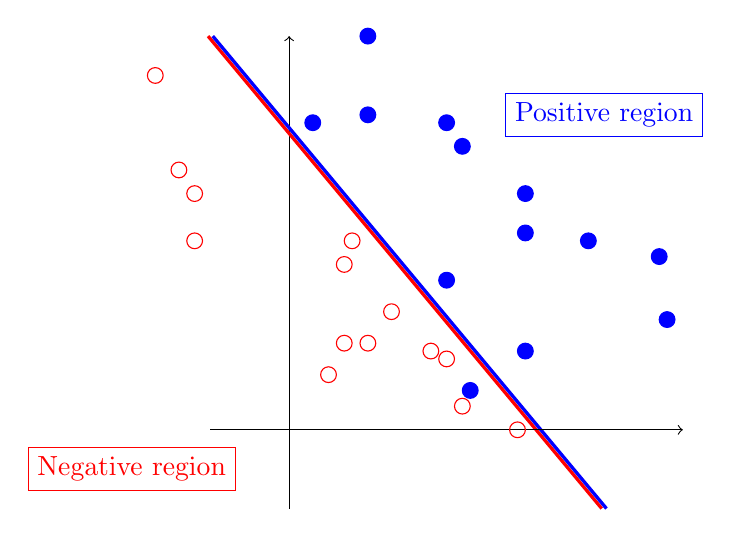
\begin{tikzpicture}
\draw[->] (0,-1) -- (0,5);
\draw[red, very thick](-1.03,5) -- (3.97,-1);
\draw[blue,very thick](-0.97,5) -- (4.03,-1);
\draw[->](-1,0) -- (5,0);
\path (-2,-0.5) node[draw,red]{Negative region};
\path(4,4) node[draw,blue]{Positive region};

\draw[blue,fill=blue] (3,3) circle(0.1cm);
\draw[blue,fill=blue] (3,2.5) circle(0.1cm);
\draw[blue,fill=blue] (3,1) circle(0.1cm);
\draw[blue,fill=blue] (2,3.9) circle(0.1cm);
\draw[blue,fill=blue] (2.2,3.6) circle(0.1cm);
\draw[blue,fill=blue] (1,4) circle(0.1cm);
\draw[blue,fill=blue] (1,5) circle(0.1cm);
\draw[blue,fill=blue] (0.3,3.9) circle(0.1cm);
\draw[blue,fill=blue] (2,1.9) circle(0.1cm);
\draw[blue,fill=blue] (3.8,2.4) circle(0.1cm);
\draw[blue,fill=blue] (4.8,1.4) circle(0.1cm);
\draw[blue,fill=blue] (4.7,2.2) circle(0.1cm);
\draw[red,fill=none] (1,1.1) circle(0.1cm);
\draw[red,fill=none] (0.7,2.1) circle(0.1cm);
\draw[red,fill=none] (2,0.9) circle(0.1cm);
\draw[red,fill=none] (2.9,0) circle(0.1cm);
\draw[red,fill=none] (0.7,1.1) circle(0.1cm);
\draw[red,fill=none] (0.5,0.7) circle(0.1cm);
\draw[red,fill=none] (2.2,0.3) circle(0.1cm);
\draw[red,fill=none] (1.3,1.5) circle(0.1cm);
\draw[red,fill=none] (1.8,1.0) circle(0.1cm);
\draw[red,fill=none] (0.8,2.4) circle(0.1cm);
\draw[red,fill=none] (-1.4,3.3) circle(0.1cm);
\draw[red,fill=none] (-1.7,4.5) circle(0.1cm);
\draw[red,fill=none] (-1.2,3.0) circle(0.1cm);
\draw[red,fill=none] (-1.2,2.4) circle(0.1cm);
\draw[blue,fill=blue] (2.3,0.5) circle(0.1cm);
\end{tikzpicture}
\caption{Linear separability.}
\label{fig:linsep}
\end{figure}

In practice, as well as in the example shown in Figure~\ref{fig:linsep},
perfect performance is rare, because real world problems are usually
not linearly separable, so some misclassifications remain, and
training is stopped when the number of remaining mistakes has stayed
stable for long enough.  When this happens, we are probably doing as
well as is possible on the training set, but does not give us
certainty about how well we will do on an unseen test set.  If the
test set and the training set are similar enough, a perceptron that
does well on the training set will also do well on the test set.
Unfortunately, we are not completely sure how similar the test set
will be, so there is an element of uncertainty in our guesses about
how well we will do.

The perceptron is an algorithm for training a \keyword{linear
  model}. The technical details of how linear models work would take
us too far afield, but the discussion of linear separability above is
part of the story.  The final weights can be understood as saying
something about the importance of each piece of evidence in a combined
solution to the classification problem. When there are a large number
of potentially useful features in a classification problem,
researchers have discovered that linear models often work well. The
perceptron algorithm is not the only way of training linear models, or
necessarily the best, but it is a good starting point for exploration.

\subsection{Modern document classification techniques}
\largerpage
The perceptron uses error-driven learning: The model reads in the training data (featurized as a vector), sends it through a series of nodes associated with weights, outputs  a prediction (spam or ham), and checks whether the prediction was correct.  If the prediction is wrong, the weights of each node are updated to move the predictions in the direction of the correct answer.

The same basic idea underlies many more sophisticated methods which have transformed language technology in recent years.  In \keyword{deep learning}, we can add intermediate layers of nodes in between the input layer and the output layer of the perceptron, to create a ``deeper'' \keyword{multi-layer network}. Such additional layers allow for more complex calculations about how different words interact with each other; for example, a multi-layer network could capture the idea that the words \exword{pain} and \exword{medicine} might be innocuous individually, but indicative of spam when they co-occur.

Such models are called \keyword{neural networks}, because the network of nodes takes inspiration from the way that firing neurons in the human brain work together to create complex behavior, and because neural networks evoke the brain's capacity for learning and abstraction.

Another way to improve our model is to use a more elaborate representation of the input features.  If we represent a document as just a bag of words, then the words \exword{pills} and \exword{medicine} have nothing in common with each other; they are each associated with a different column of a term-by-document matrix.  But we are obviously missing a key insight here -- \exword{pills} and \exword{medicine} have somewhat similar meanings.  How do we know?  They are not strictly synonyms, but they can be used in similar contexts -- \exsent{take some pills}, \exsent{take some medicine}; \exsent{pain pills}, \exsent{pain medicine}.  We saw in \chapref{ch:textasdata} that we can represent words as vectors such that words occurring in similar contexts, such as \exword{pills} and \exword{medicine}, have similar vectors.


In fact,  \textit{pills} and \textit{medicine} have similar meanings and co-occurrence patterns not just in  spam/ham emails, but also in English text as a whole.  So, rather than just capturing what words pattern similarly within our specific dataset, we might want to use \keyword{pre-trained} word embeddings that were built on a large amount of general-purpose English text (for example, Wikipedia), and feed that information into our model alongside a small set of labeled spam and ham emails.  That way, our model has access to a lot of general information about English in addition to specific information about spam and ham.  This strategy is called \keyword{transfer learning}: Our model is given some useful general information, such as the fact that \exword{pills} and \exword{medicine} have similar meanings, and transfers it to the specific task of spam detection. 


In 2018, the idea of pre-training and transfer learning was taken to a new extreme when a team at Google (led by Jacob Devlin) released a model known as \keyword{BERT} \citep{Devlin-etal:2019}.  Rather than just capturing information about which words are similar to each other, BERT was designed to represent a massive quantity of information about English-language text, which can be transferred to a variety of specific tasks, including text classification. 

BERT is a neural network that is originally trained to do two specific tasks, (i) masked word prediction and (ii) next sentence prediction, using a huge amount of data, such as the whole of English-language Wikipedia.  In \keyword{masked word prediction}, the researchers randomly blanked out 15 percent of the words in the text (illustrating here with a sentence from the English Wikipedia page on lions), and trained the model to choose the right word to fill in the blank.  In other words, in the pre-training phase, the model makes a prediction, then checks to see if the prediction matched the original Wikipedia text, and then updates its weights to do better next time, until it gets very good at filling in the blanks of sentences.

\ea  One of the most --- recognised animal symbols in human culture, the lion has --- extensively --- in sculptures and paintings, on national ---, and in contemporary --- and literature.
\z


How would you fill in these blanks?  More importantly, what knowledge do you draw on to make an educated guess?  (The missing words are \exword{widely, been, depicted, flags,} and \exword{films}.)


You probably considered the words immediately to the left and right of the blank, but also other words in the sentence, its structure, and its overall meaning.  To fill in the word \exword{depicted}, you may have considered that the syntactic context requires a past participle, and that depictions are related to symbols and paintings. We already saw in \chapref{ch:call} that such fill-in-the-blank exercises are also used to test the knowledge of human language learners.  By learning to fill in the blanks correctly, the idea is that BERT approximates that same knowledge.  



In \keyword{next sentence prediction}, the researchers randomly paired some sentences with the sentence that actually comes next in the text, and paired other sentences with a randomly chosen sentence from elsewhere in the data (again illustrating with Wikipedia text).  The model was trained to decide whether a given pair of sentences indeed occur next to each other or not.  In a sense, this is a text classification task -- the model is given a two-sentence text and classifies it as either cohesive or disjointed.

\ea Typically, the lion inhabits grasslands and savannas, but is absent in dense forests. // It is usually more diurnal than other big cats, but when persecuted it adapts to being active at night and at twilight.



\ex Typically, the lion inhabits grasslands and savannas, but is absent in dense forests.  // Despite the name, shellfish are not actually fish, but are simply water-dwelling animals.

\z 

How would you decide which sentences match and which do not?  What knowledge do you use?   (The sentences about lions indeed occur next to each other in Wikipedia; the sentence about shellfish is from a different page.) You probably thought about how the pronoun \exword{it} could refer back to the singular noun \exword{lion}; how \exword{cats} are related to lions, how the daily habits of an animal might be described in the same paragraph as its habitat, and how shellfish, fish, and water are not particularly related to the lions, savannas, and forests discussed in the prior sentence.  By learning to decide which sentences match, the idea is that BERT approximates that same knowledge. 

Stepping back, why would researchers take the trouble to train a network to fill in blanks and to decide whether two sentences go next to each other?  These tasks are not particularly useful in a commercial context!

One major advantage of these tasks is that the labels required for training -- the missing words and the contiguous sentences -- are already provided by the text itself, unlike human labels for ham and spam, so it is easy to train BERT on a massive amount of text.  The other major advantage is that these tasks require BERT to ``learn'' a great deal of rich information about English text, both at the word level and the sentence level.  For example, BERT will learn that \exword{pills} and \exword{medicine} are similar because they are both often good candidates to fill in the same missing word in a sentence.  Moreover, masked word prediction leads BERT to represent not just the overall distribution of a word type such as \exword{pills}, but the context of each word token -- the fact that \exword{pills} means something different in a sentence like \exsent{This sweater pills in the wash} versus \exsent{Take these pills for your headache}.  Each token of \exword{pills} receives a different vector representation.

Even if masked word prediction and next sentence classification are not particularly useful on their own, the idea is that they serve as a powerful pre-training regimen.  Instead of just importing pre-trained word embeddings into a spam-detection model, the idea is that we can read in the entire BERT network, pre-trained on masked word prediction and next sentence prediction, and then add a few layers on top of it which we train on labeled spam/ham data to do spam detection (known as \keyword{fine-tuning} BERT's pre-trained knowledge for this specific task).  This way, the model will not only have access to a small set of spam/ham data, but is also able to transfer a massive amount of general information about English.  The use of such general information is known as \keyword{transfer learning.}


To use a sports analogy,  imagine that you want to train, as  efficiently as possible, to compete at many different speed sports.  (BERT is trained, as efficiently as possible, to compete at many different language-related tasks). You decide to focus on push-ups and squat jumps.  (BERT focuses on masked word prediction and next sentence prediction.) These exercises are easy to do anywhere, requiring no  specialized equipment (for BERT, these tasks require no  specialized labels).   They are also very challenging exercises that work out your entire body, your muscles and your cardiovascular system, explosiveness and endurance (for BERT, these tasks require knowledge about the structure, meaning, and statistical tendencies of English text). You do an enormous number of push-ups and squat jumps,  several hours a day for months (BERT trains on masked word prediction and next sentence prediction on an enormous amount of data.)  Once you have trained to be very good at push-ups and squat jumps, you will still need specialized practice to compete at sports such as running, swimming, or rowing (BERT still requires some fine-tuning to do spam detection using labeled spam/ham data.)  But the athleticism developed from push-ups and squat jumps is highly transferable, and this training regimen has made you a powerful, versatile athlete well-prepared to succeed at many different sports.  (The information gleaned from masked word prediction and next sentence prediction is highly transferable, and BERT's training regimen has made it a powerful, versatile  representation of language well-prepared to succeed at many different tasks.)

Using the power of transfer learning, BERT and its descendants form the basis of modern document classification, and in many tasks such models are stunningly accurate.




\subsection{Which classifier to use?}

We have toured many different techniques for classifying documents, walking through the simple examples of naive Bayes and the Perceptron, and then sketching the intuition used in the elaborate models of today.  With so many options, which one should you use?

Coming back to our medical discussion of payoffs and priorities, it depends on what you are trying to do.  If your goal is to get the best performance, and if you have time and programming skills, you may want to use a model such as BERT that leverages transfer learning.  If you are intellectually curious  about which specific words are most associated with which labels, you may want to use naive Bayes, which can show you the spam:ham odds ratio associated with a particular word; thanks to its simplicity, naive Bayes is  more \keyword{interpretable} than more elaborate techniques.  You may also want to try out a simple model and see how well it does as a baseline, and then decide if you need something more complex.

To get started on a practical level, you might use the Pandas library in Python to format your data as a matrix (expect to spend some time on such formatting!), and Google's TensorFlow package in Python to try out different machine learning techniques.  If you search the web, there are lots of resources and sample code notebooks to help you get started.



% The main reason for including brief discussion of the perceptron is to show that there is more than one way to do machine learning. Intuitively, the idea of collecting statistics over a collection of examples is very different from maintaining a collection of weights that are updated in a mistake-driven way. But at a deeper level, both of these approaches are supervised learning, and it is likely that they will perform similarly a lot of the time. Usually, the most important part of a machine learning solution is the choice of features that provide information about the distinctions that we want the classifiers to learn about, and the choice of which classifier plays an important but secondary role. Our advice is to try a few off-the-shelf classifiers and choose the one which seems to be working best for your problem. A toolkit containing state-of-the-art implementations of many classifiers is Weka (\url{http://en.wikipedia.org/wiki/Weka_(machine_learning)}), which is written in the programming language Java and is fairly easy to use.

%Weka also contains software for predict numeric continuous values, such as the numbers of stars in a movie review (here we are imagining that the movie review site produces really detailed ratings, not just whole numbers of stars, and that the rating could be a decimal like 3.72) .  Predicting continuous values from features is called \keyword{regression}. By contrast, the perceptron and Naive Bayes produce predictions from a fixed set of discrete values, often just \emph{yes} or \emph{no}. Programs that predict discrete values are called \keyword{classifiers} in the machine-learning literature, and the term \keyword{classification} is used when it is important to make clear that they are predicting discrete rather than continuous values.

% Another way of making our general point is that the choice of classifier should be based on thinking about the \keyword{context of use} of the technology. While programmers will certainly care about the details of how the algorithms work, users and managers will care more about what the system can do, what kind of errors it will make, and how this fits in with the real world needs of the organizations or other clients who want to use the technology. One of the reasons for the substantial emphasis on evaluation in this chapter is that good evaluation focuses attention on the tradeoffs that are involved in really using technology.  In the final section of this chapter, we provide a brief case study to illustrate how document classification technology is actually deployed.  The important lesson is not that the authors think the technology is cool, although we do think it is, but that we think that it is useful for finding good solutions to real-world problems.

\section{Some other applications  of machine learning}

Stepping back, machine learning is a remarkably powerful idea with important applications far beyond text classification.  Classification -- mapping a vector of features to a label, chosen from a finite set of possible labels -- is also used in computer vision, where we can represent an image as a vector of pixels and learn how to label it as a cat or a dog, or perhaps learn to map an image of a handwritten digit to the number (0, 1, 2, 3, 4, 5, 6, 7, 8, or 9) that it represents.  We can also represent a credit card transaction as a vector of features (the time of day, the type of store, the location, the price, information about the cardholder's usual habits) and learn to label it as fraudulent or legitimate.  And so on.

As we mentioned above, classification is an example of \keyword{supervised learning}, because we give the computer some ``right answers'' (correctly labeled spam/ham emails) and train it to generalize those labels to new data.  Apart from classification, the other main type of supervised learning is \keyword{regression}; there, instead of a label, our goal is to predict a continuous numerical value. To use a language example, we could train a model to read an essay and give it a score out of 100.  Here, too, the model learns to generalize from ``right answers'', but these would take the form of featurized essays that have already been correctly scored.  (Before we turn this model loose on real student work, we would want to make sure that it was not reproducing some sort of bias that could give unfairly low scores to certain students!)  We could also represent a house as a vector of features (its location, square footage, year it was built, number of bathrooms) and learn to predict its price.  And so on.

In contrast, \keyword{unsupervised learning} is used when we do not give the model any ``right answers'' -- because we do not have the resources to collect labels, or because we do not even know what such labels would be.  We saw an example of unsupervised learning in \chapref{ch:textasdata} in the context of topic modeling: A topic modeling algorithm is not given any labels to generalize, but is instead designed to identify meaningful groups of words and documents (each associated with topics) in a bottom-up manner.  Another type of unsupervised learning is called \keyword{clustering}, in which a model is asked to group similar data points together -- for example, clustering together documents that are similar to one another according to some sort of vector representation of the words used therein.   (Outside of text, we could also cluster together similar images, similar houses, and so on, as long as these are represented as vectors.)  With no need for expensive labels, clustering is useful for exploring a large dataset that you do not have time to read.  The model does not give names to the clusters (although a human reader may try to), and the main disadvantage is that the clusters may not be intuitive; perhaps it would put some social emails into a cluster dominated by work emails, if the social emails happen to mention calendar dates.

We hope that this brief overview has offered a framework to understand the power of machine learning, which will come up again in this book and perhaps in your life more broadly.

% The reader will be able to notice that articles in a given cluster share something, such as being about sports, but the algorithm would be just grouping articles, not trying to name the clusters. The big plus of this approach is that you do not need a training set, so there is no costly process of going through labeling up the articles. The big negative is that the clusters might not be that intuitive. For example, if you cluster common words, one cluster often turns out to be the words \exsent{Monday}, \exsent{Tuesday}, \exsent{Wednesday}, \exsent{Thursday}, with \exsent{Friday} off in another cluster. This is because Friday is the only weekday that frequently turns up following \exsent{Thank goodness it's \ldots}.


% reinforcement learning.....
% video games?, robots????,
% intelligent behabior in complex environments
% agent, environment, reward, state
% policy gradients.... 
% needs to learn a policy for acting in various environments to get the best reward.
% state, action, reward.
% if something works, you do it slightly more often - you update your policy gradient.
% but maybe if a reward requires MANY different actions in sequence, you will never get there randomly, 
% or you will never know where you went wrong if you fail (maybe you did a lot right, but you may not know that) - `credit assignment problem'
% can also build in interim rewards, that are not the final reward???? `reward shaping???'
% but takes a lot of work
% reinforecement learning is hard. 
%
% action affects environment, environment affects state, state affects action
% action also leads to a reward.... 
% given a certain state, what action is likely to lead to a reward
% try a few different things, see what works -- exploration


% what is reinforcement learning
% need to add in somewhere about OVERFITTING.... 
% WHAT HAPPENED TO THAT PART, add it back in

%

\section{Sentiment analysis}

With this background, we can come back to another key application of text classification -- classifying texts by their emotional valence, also known as \keyword{sentiment analysis}.

On websites such as IMDB (Internet Movie DataBase) and Amazon, people can write a review of a movie or product, and  annotate it with a star rating: 5/5 or 10/10 stars if they love it, 0 stars if they hate it -- helpfully providing labels for those of us interested in sentiment analysis!  Drawing on our discussion of machine learning, we could train a regression model to predict a review's star rating out of 10, or train a classifier to assign a label of positive or negative (or perhaps positive, negative, neutral).

Here are two IMDB reviews for \exword{Parasite} (2019), the first Korean film to win Best Picture at the Academy Awards.  Without knowing the star rating, what clues do you use to figure out whether each review is positive or negative?

\ea The most original film of 2019 and it is wickedly funny and darkly disturbing all at the same time. Class warfare at its best.


\ex  I truly don't know what I missed but this was just not my cup of tea (or my mom's) and it felt unnecessarily gruesome and strange rather than masterful and sharp. Instead of awaiting the next moment with excitement and suspense, I found myself cringing at the actors' performances as they weren't believable and was confused at how poorly-written the dialogue was. 

\z 

 The first review is positive (10/10 stars), and the second review is negative (1/10).  The positive review uses positive words -- \exword{original, funny, best} -- along with the slightly negative word \exword{disturbing}; it also uses superlatives (\exword{most, best}) and intensifiers (\exword{wickedly,  darkly}).  The negative review uses some negative words -- \exword{strange, cringing, poorly-written}.  It also uses some positive words (\exword{masterful, sharp, excitement, suspense, believable}), but some of them are negated by \exword{instead of} and \exword{weren't}.  In fact, as shown by \citet{Potts:2010} and discussed in \chapref{ch:textasdata}, negation itself (\exword{don't, not, unnecessarily, weren't}) is common in  negative reviews as a whole, which is intriguing because you might have expected negation to have a purely logical meaning rather than an emotional one.


Just as with spam detection, we can feed labeled positive/negative reviews into a classifier (naive Bayes, the Perceptron, or a fancy classifier using transfer learning) and train it to classify the sentiment of future reviews.  The classifier will probably be more accurate if it ``knows'' that most of the positive words in the negative review are semantically negated.  One quick-and-dirty technique \citep{DasChen:2007} is to prepend \exword{NOT} to every word that falls between negation and the end of a sentence or clause -- \exsent{they weren't NOTbelievable} -- before making a bag-of-words.  This way, \exword{believable} and \exword{NOTbelievable}  count as two different words, one of which probably predominates in positive reviews, the other in negative ones.  On reviews like the two we just read, a classifier should be quite accurate.

In addition to measuring the accuracy of our classifier, it is also worthwhile to examine the documents that it classifies incorrectly (\keyword{error analysis}).  Such hard-to-classify documents may illuminate interesting subtleties in the data, and help us understand what the classifier ``knows'' and doesn't ``know''.  

For example, we tried one classifier that was correct about the positive and negative reviews discussed above, but still mis-classified as positive a review from the legendary film critic Roger Ebert which is actually humorously negative:



\ea  The director [of the 2004 film \exword{Catwoman}], whose name is Pitof, was probably issued with two names at birth and would be wise to use the other one on his next project.
\z 





To do an error analysis, we can ask ourselves:  

\begin{itemize}

\item \emph{Why is this review difficult to classify?} Most likely, because it does not use any negative-sentiment words; the negative opinion is inferred by complex hypothetical reasoning.  To understand why the \exword{Catwoman} review is negative, we have to understand that the director would want to use another name on his next project because the  project with his original name was bad; but that logic is not spelled out in the review itself.

\item \emph{What do these errors tell us about the subtleties of our data?} This review shows that language is complicated! Negative sentiment does not just come from negative words, but also arises when sentiment-neutral language is used to describe a state of affairs that we recognize extra-textually as negative.
 

\item \emph{What do these errors tell us about what the classifier ``knows'' and doesn't ``know''?}  The classifier performs well on reviews that state their sentiment outright in words, but does not fully capture the complex extra-textual reasoning required to decode Ebert's snark.

\end{itemize}

Just like spam filtering, sentiment analysis can be used for practical purposes, for example, to track consumers' sentiment towards one's company on social media.  But it can also be used for purely intellectual explorations in the areas of digital humanities, computational social science, and corpus linguistics introduced in \chapref{ch:textasdata}.  Within digital humanities, one could track the sentiment of sentences in a novel from beginning to end or the sentiment of sentences about various characters.  In computational social science, one might explore the sentiment of news articles or statements by politicians across the ideological spectrum.  In corpus linguistics, one could explore how a word's sentiment (or that of its collocational context) might change over time in historical data, as when the word \exword{mistress} changed from meaning ``Mrs.'' to meaning ``a woman in an extramarital affair'' \citep{TraugottDasher:2001}.  Returning to the theme of how computers can extract meaning from text,  sentiment analysis represents one way that computers can capture emotional meaning.

% talk about how it is also important to do ERROR ANALYSIS
% this will help us understand the classifier and why it is doing what it is doing
% what is hard and why?
% add in the thing about overfitting too.
% 

\begin{tblsfilledsymbol}{\underthehoodsubsection{Benchmarks and leaderboards in NLP}}{glass}
\begin{underthehood}

BERT was recognized as a striking advance because it shot to the top of various \keyword{leaderboards} tracking performance on various \keyword{benchmarks} in natural language processing.  These benchmarks represent standardized tests, similar to the Scholastic Aptitude Test (SAT) used for college admission in the United States,  designed to test difficult tasks in language understanding.  Just as the SAT publicizes practice problems but not the real test that students are graded on, these benchmarks provide training data but evaluate models for their performance on an unseen test set.  Moreover, similar to how SAT measures quantitative and verbal skills in the same test, a \keyword{combined benchmark} brings together several different tasks into a unified scoring framework.  The creators of such benchmarks also gather human annotations from web platforms such as Mechanical Turk to compare for the models' performance.

Such benchmarks are common in computer science; in the field of computer vision, the ImageNet benchmark \citep{Deng-etal:2009} tests models for whether they can correctly assign text labels (\exword{strawberry, dog}) to images.  It took about seven years for computers to compete with human performance on the ImageNet data, but recent progress has accelerated.  In NLP, it took only one year for the combined GLUE (General Language Understanding Evaluation) benchmark of \citet{Wang-etal:2018} to be deemed too easy for models such as BERT, motivating the more difficult SuperGLUE version \citep{Wang-etal:2019}.  

SuperGLUE brings together eight different tasks meant to test a model's ability to reason about English text.  For example, drawn from \citet{Dagan-etal:2005}, the RTE (Recognizing Textual Entailment) task asks whether \REF{reagan} entails \REF{normandy} (it does not).  


\ea \label{rte} \ea \label{reagan} Reagan attended a ceremony in Washington to commemorate the landings in Normandy. 
    \ex \label{normandy} Washington is located in Normandy. [False; not entailed.]
    \z
    \z 


In fact, there are two different routes to the correct answer in \REF{rte}.  Leveraging knowledge about events, one could reason that a ceremony can take place in a different location from the event it commemorates.  Or one could use the geographical fact that Washington is in the United States while Normandy is in France.  So perhaps \REF{rte} is too easy!

To make more difficult benchmarks, some researchers gather \keyword{adversarial} examples, explicitly asking gig workers to try to fool the model.  The adversarial example \REF{adversary} is tricky for a model of textual entailment   \citep{Nie-etal:2020} because it requires the model to infer that the \exword{assassination} of a journalist entails \exword{another individual laid waste to} him -- requiring complex reasoning about how the abstract event-denoting noun \exword{assassination} can be paraphrased by a sentence using an obscure idiom (\exword{laid waste to}).


\ea \label{adversary} 
    \ea \label{roberto} Roberto Javier Mora Garc\'ia (c. 1962 – 16 March 2004) was a Mexican journalist and editorial director of \exword{El Ma\~nana}  [\ldots] prior to his assassination.
    \ex  \label{waste} Another individual laid waste to Roberto Javier Mora Garc\'ia. [True; entailed.]
\z
\z 

Benchmarks are important for measuring progress and challenging the research community to improve.  But like any standardized test, they have been criticized.  For one, SuperGLUE (General \emph{Language} Understanding Evaluation)  only really measures \emph{English} understanding, further cementing English as a hegemonic standard.  Moreover, as argued by \citet{EthJurafsky:2020}, benchmarks ignore progress on other important dimensions such as fairness (avoiding social biases) or compactness (aiming for smaller, more energy-efficient models).  They don't necessarily reward the theoretically interesting insights or explanations sought by linguists.  Because NLP benchmarks prioritize objective true-or-false questions, they do not extend easily to models offering open-ended language generation.   Therefore, each researcher has to decide for themselves how much they prioritize benchmarks versus other definitions of success.


\end{underthehood}
\end{tblsfilledsymbol}



\section{Consequences}


Some challenging text classification tasks are not commercially applicable, but still provide insight into the power and limits of classifiers, and the subtleties of the information conveyed in language.  What accuracy would you expect from a classifier that tries to predict whether a comment is sarcastic or serious (perhaps using as labels the \exword{/s} symbol that some web writers use to convey sarcasm)? What about a classifier that reads narratives on the Reddit web forum r/AmITheAsshole, where people describe their conduct and ask readers for a moral judgment, and tries to predict whether a person is deemed to be ``the asshole'' or ``not the asshole''?  What about a classifier that reads sentences and tries to label them as ``grammatical'' or ``ungrammatical'' following the labels used in linguistics textbooks \citep{Warstadt-etal:2019}?  By comparing human and computer performance  on such tasks, we learn more about the ``intelligence'' of both humans and computers, as well as the subtleties of these data.

Other text classification tasks pose challenging ethical questions.  What if you tried to  detect automatically which job candidates should get an interview based on their r\'esum\'e, training on previously submitted r\'esum\'es of people who were or were not interviewed?  For a company that receives thousands of   r\'esum\'es a day, many tedious hours of human labor could be saved by automating this process.  But what if the classifier learns that the word \exword{lacrosse} increases a person's chance of an interview, or that the word \exword{community college} decreases it, when neither of these socio-economic signals actually relates to the job description?  Our system could end up reproducing harmful inequalities.  (Would a human be any less biased?  How could the performance of both human and automated r\'esum\'e-screeners be made anti-discriminatory?)

Moreover, how does text change when its authors know that it will be run through an automatic classifier? How do spammers adjust spam to slip through spam filters? How do job applicants tailor their r\'esum\'es to pass automatic screenings?  How might such classifiers need to be updated to account for these new strategies?


Armed with the basics of machine learning and its application to document classification, you have a powerful set of tools for understanding the world.  But you also have to think critically about linguistic complexity, human priorities, and ethics in deciding how to apply these tools.


\begin{tblsfilledsymbol}{Checklist}{test}

\begin{itemize}
\item Give examples of text classification tasks.  
\item Brainstorm several business applications of text classification.
\item Give examples of other classification tasks beyond the realm of documents.
\item Explain specificity, sensitivity, and their relevance for text classification.
\item Discuss what constitutes ``success'' for a classifier, using quantitative notions such as sensitivity and specificity as well as  one's qualitative priorities.
\item Explain base rates and the base rate fallacy.
\item Define over-fitting and its significance for machine learning.
\item Explain how naive Bayes classification works.
\item Explain how the Perceptron classifier works.
\item Sketch the idea of transfer learning.  
\item Describe the two tasks used to train BERT and explain why they were used.
\item Distinguish supervised versus unsupervised learning.
\item Analyze which tasks and examples you would predict to be easier or harder for a classifier. 
\end{itemize}
\end{tblsfilledsymbol}



\begin{tblsfilledsymbol}{Exercises}{pencil}
    


\begin{enumerate}

\item  Expanding beyond consumer technology such as spam filters, think back to digital humanities and computational social science as discussed in \chapref{ch:textasdata}.  How can classification tools be used in these realms?  To help you get started, consider how you might train a classifier to label text for its genre; its sentiment; its author (out of a closed class of authors); or for its author's gender, political party, or native language.  How would you find such labels to train your classifier?  To what extent do you think that a classifier could learn to predict these labels from the text?


\item  Sentiment analysis makes use of user-provided training labels; users annotate their own review with a star indicating its sentiment.  What other sorts of user-provided labels are available in online text today? How could they be used?



\item  Many advertisements and mass mailings probably make it into your inbox rather than your spam folder.  Do you consider these emails to be spam or ham (or something in between)?   How do you think an email system should handle them?


\item 
  \begin{enumerate}
\item Table~\ref{tab:payoffs} gives a calculation of the payoffs associated with each outcome of the medical test in the extended example. Put this together with the population statistics in Table~\ref{fig:diagnostic3}
to calculate the overall payoffs from: (a) always running the test, and (b) never running the test. Which is the more cost-effective policy for the hospital ? 
\item We carefully set up our example so that everyone was cured and the only effect of your decision is financial, but of course the mathematics also applies to decisions where much more is at stake. 
Now that you have learned about false positives, true positives, payoffs and the rest, you have the conceptual tools to understand the tradeoffs that are involved in deciding whether a country should
have a policy of offering mammography as a general screening tool for breast cancer. We recommend that you find information about this online, read about it, and see what you think. Do not
stop after the first article you read. It is a controversial issue, and you will find sensible articles advocating both for and against general screening. 
\end{enumerate}

\item  You are the owner of a spam filtering service: 

\begin{enumerate}
\item
Currently, your server gets 2000 spams per hour and only 500
good messages. The filter classifies 95 percent of the spams correctly, 
and misclassifies the other 5 percent. It classifies 99 percent of the good
messages correctly, and misclassifies the other percent.
Tabulate the results: How many false positives and how many false
negatives do you expect to see each hour?
Calculate 
 the precision, sensitivity, and specificity of the spam 
filter.
\item
You receive word
that a criminal gang is planning to double the amount of spam that it
sends to your server. There will now be 4000 spam messages per hour
instead of 2000. The number of good messages stays unchanged at 500.
In your marketing literature, you have quoted
the precision, recall, sensitivity and specificity of your spam
filter. You assume that the misclassification rates will stay the
same (5 percent for spam, 1 percent for good messages).
Should you put in a call to the technical writing department
warning them that the literature will need to be revised? Why or why
not? And if so, what will need to be revised?
\end{enumerate}

\item  Continue the calculation from Section \ref{sec:nb}.
	 Assume that the next word in the email is \exsent{cookie}. Using the frequency statistics from Table~\ref{spam:data},
	carry out the next step of the calculation. What is the cumulative ratio for spam/non-spam?

\item  Your colleague labels product reviews (\exsent{Sturdy and comfortable, this cot folds up and out of sight with minimal effort}) based on the gender of the review's author, mapping the author's self-disclosed name (\exword{Sarah, Ralph}) to census data about the likely gender of people with that name.  Your colleague then trains a classifier to label reviews for the gender of the author.  The colleague's goal is to label the author gender of anonymous reviews, which could provide demographic marketing data to sellers.  What comments would you offer this colleague -- about the difficulty of the task, the assumptions underlying it, and the real-world utility of the classifier?
	

\item   Read some posts on Reddit/AmITheAsshole and discuss what knowledge would be required to correctly label the author as ``the asshole'' or ``not the asshole''.  Do you think that modern LLMs will succeed at this task? Can you search the literature for recent discussion or try to test this prediction yourself?
	

\item  Try out some web demos of sentiment classifiers -- you can find the most up-to-date ones by searching the web for \exsent{sentiment analysis demo} -- and try to ``break'' the classifier by giving it difficult examples.

\end{enumerate}
\end{tblsfilledsymbol}



\begin{tblsfilledsymbol}{Further reading}{book}
    
The statistical approach to spam filtering was popularised by Paul Graham's ``A Plan for Spam''.\footnote{\url{https://www.paulgraham.com/spam.html}, accessed 2024-04-18.} His article, which has aged very well, is an excellent starting point for learning about the technology and sociology of spam.  
  
  \citet{DBLP:journals/ftir/PangL07} offers a comprehensive introduction to opinion-mining and sentiment analysis. 
  
  The discussion of base rate fallacy is based on \citet{BarHillel:80}. Cognitive biases are discussed in the literature on psychology and behavioral economics.  
  
  On websites such as YouTube, Medium, and GitHub, you can find many excellent tutorials and example code about sentiment analysis, document classification,  transfer learning, and BERT.

\end{tblsfilledsymbol}
